\section{Preface}
\label{sec:preface}

Imagine being the owner of a piece of technology. It can be any physical device. Without maintenance, it is unavoidable that, after a certain amount of time of usage it will have some sort of malfunction.
To overcome this problem, usually, maintenance work is planned and performed by a team of skilled technicians. 

The simplest way of executing maintenance is to fix the device when it breaks. This is called \emph{reactive maintenance} (\gls{rm}). This has been done since forever, and it is still a very popular approach today, but it has numerous drawbacks, including extended downtime for repairs and logistical challenges associated with spare parts.

The other family of maintenance techniques is called \emph{preventive (or proactive) maintenance} (\gls{pvm}). All those techniques share the property of being applied before the device shows a malfunction. This is a very broad category, and it includes a lot of different techniques, most of which will be described in \autoref{ch:state_of_the_art}.

Back to the example, the owner of the device may want to avoid fixing it when it has already failed as much as possible, so the first improvement could be to perform maintenance periodically (on a schedule). This is called \emph{predetermined maintenance}, and it is the simplest approach to \gls{pvm}. It's basically the same approach that every motorist uses to minimize the risk of the vehicle breaking down in the middle of the road. 
The owner may want to take the technique a step further and seek some sort of guidance on deciding when to perform maintenance. A very intuitive approach is to simply ask the skilled technicians to inspect all the devices very often to try to understand if something is wrong without interfering with the normal operation of the device.

If a technician has enough experience, he may be able to detect the vast majority of the problems before they become critical. He may do that simply using his senses, for example by listening to the sound of the device, or by touching it to feel how much it vibrates, how hot is it and so on. 

\maskk{I would like to share, as a real-life example, what I witnessed during the commissioning of a new power plant. I remember that the commissioning manager (that is a chemist) was able to detect if the demineralization unit was working properly or not by simply tasting the water it produced before the necessary instruments were installed.}

This naive approach can be enhanced by using a large number of sensors to monitor the most critical parameters of the device. In this case, the technician will train himself more on the data of the sensors, rather than on inspecting the device directly. 

At this point, the next logical step would be to use the data from the sensor to train an algorithm, that will detect some patterns in the data that are not easily detectable by a human. This is called \emph{condition-based maintenance} (\gls{cbm}). This is the most common approach to \gls{pm} today. If this algorithm is trained only on the data taken when the device is working properly, it would only be able to detect a novel behaviour, this is called \emph{novelty detection} (\gls{nd}). If the algorithm is trained on both the data taken when the device is working properly and the data taken when the device is malfunctioning in a specific way, it would be also able to detect the specific malfunction, this is called \emph{fault detection} (\gls{fd}).

One last improvement to the \gls{cbm} approach is to use an algorithm that will also try to predict how much time is left before a critical malfunction will occur. This approach is referred to as \emph{predictive maintenance} (\gls{pdm}). This is the most advanced approach to \gls{pm} today.

Both \gls{cbm} and \gls{pdm} could be done by using a model of the system that will predict the future behaviour based on the current state of the system. The problem with this approach is that it is very difficult to build a model that is accurate enough to be useful. Most of the time, in industrial applications, such a model is not available.
A workaround to this problem is to apply an Unsupervised Machine Learning (\gls{uml}) algorithm to the sensor data. This has the advantage of not needing a model of the system, but it has the drawback of being a black-box approach, so the parameters of the algorithm are not easily interpretable in a physical sense. Furthermore, the algorithm will be fairly good at detecting anomalies, but it will have some limitations in predicting the future behaviour of the system since it will likely be based on a forecast done interpolating the data of the past.

\paragraph*{}
To visualize this evolution of maintenance approaches, let's have a look at \autoref{fig:earlysteamengine}. This is a purely mechanical device, so the only way to detect a malfunction before it causes a failure is by trusting the \quoted{gut feeling} of the operator. Moving on, the device in \autoref{fig:modernsteamengine} is also a steam engine, but it is equipped with some analogue gauges. In this case, it is possible to define some thresholds for the readings that are indicative of a malfunction and look at the time evolution of the values. The measure of the sensor is immediately displayed to the operator. Moving into nowadays, the device in \autoref{fig:controlroom} is a state of the Art control room. The data from the sensors are elaborated by a computer and displayed to the operator on screens. This allows the computer to run algorithms on the sensor data.

\begin{figure}
    \centering
    \begin{subfigure}{0.3\textwidth}  % <----
        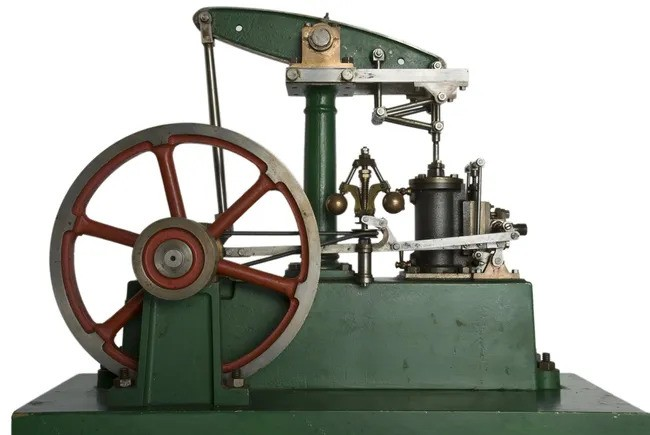
\includegraphics[width=\textwidth]{images/Intro/earlysteamengine.jpg}
        \caption{early steam engine \cite{steam_engine}}
        \label{fig:earlysteamengine}
    \end{subfigure}
    \begin{subfigure}{0.3\textwidth}  % <----
        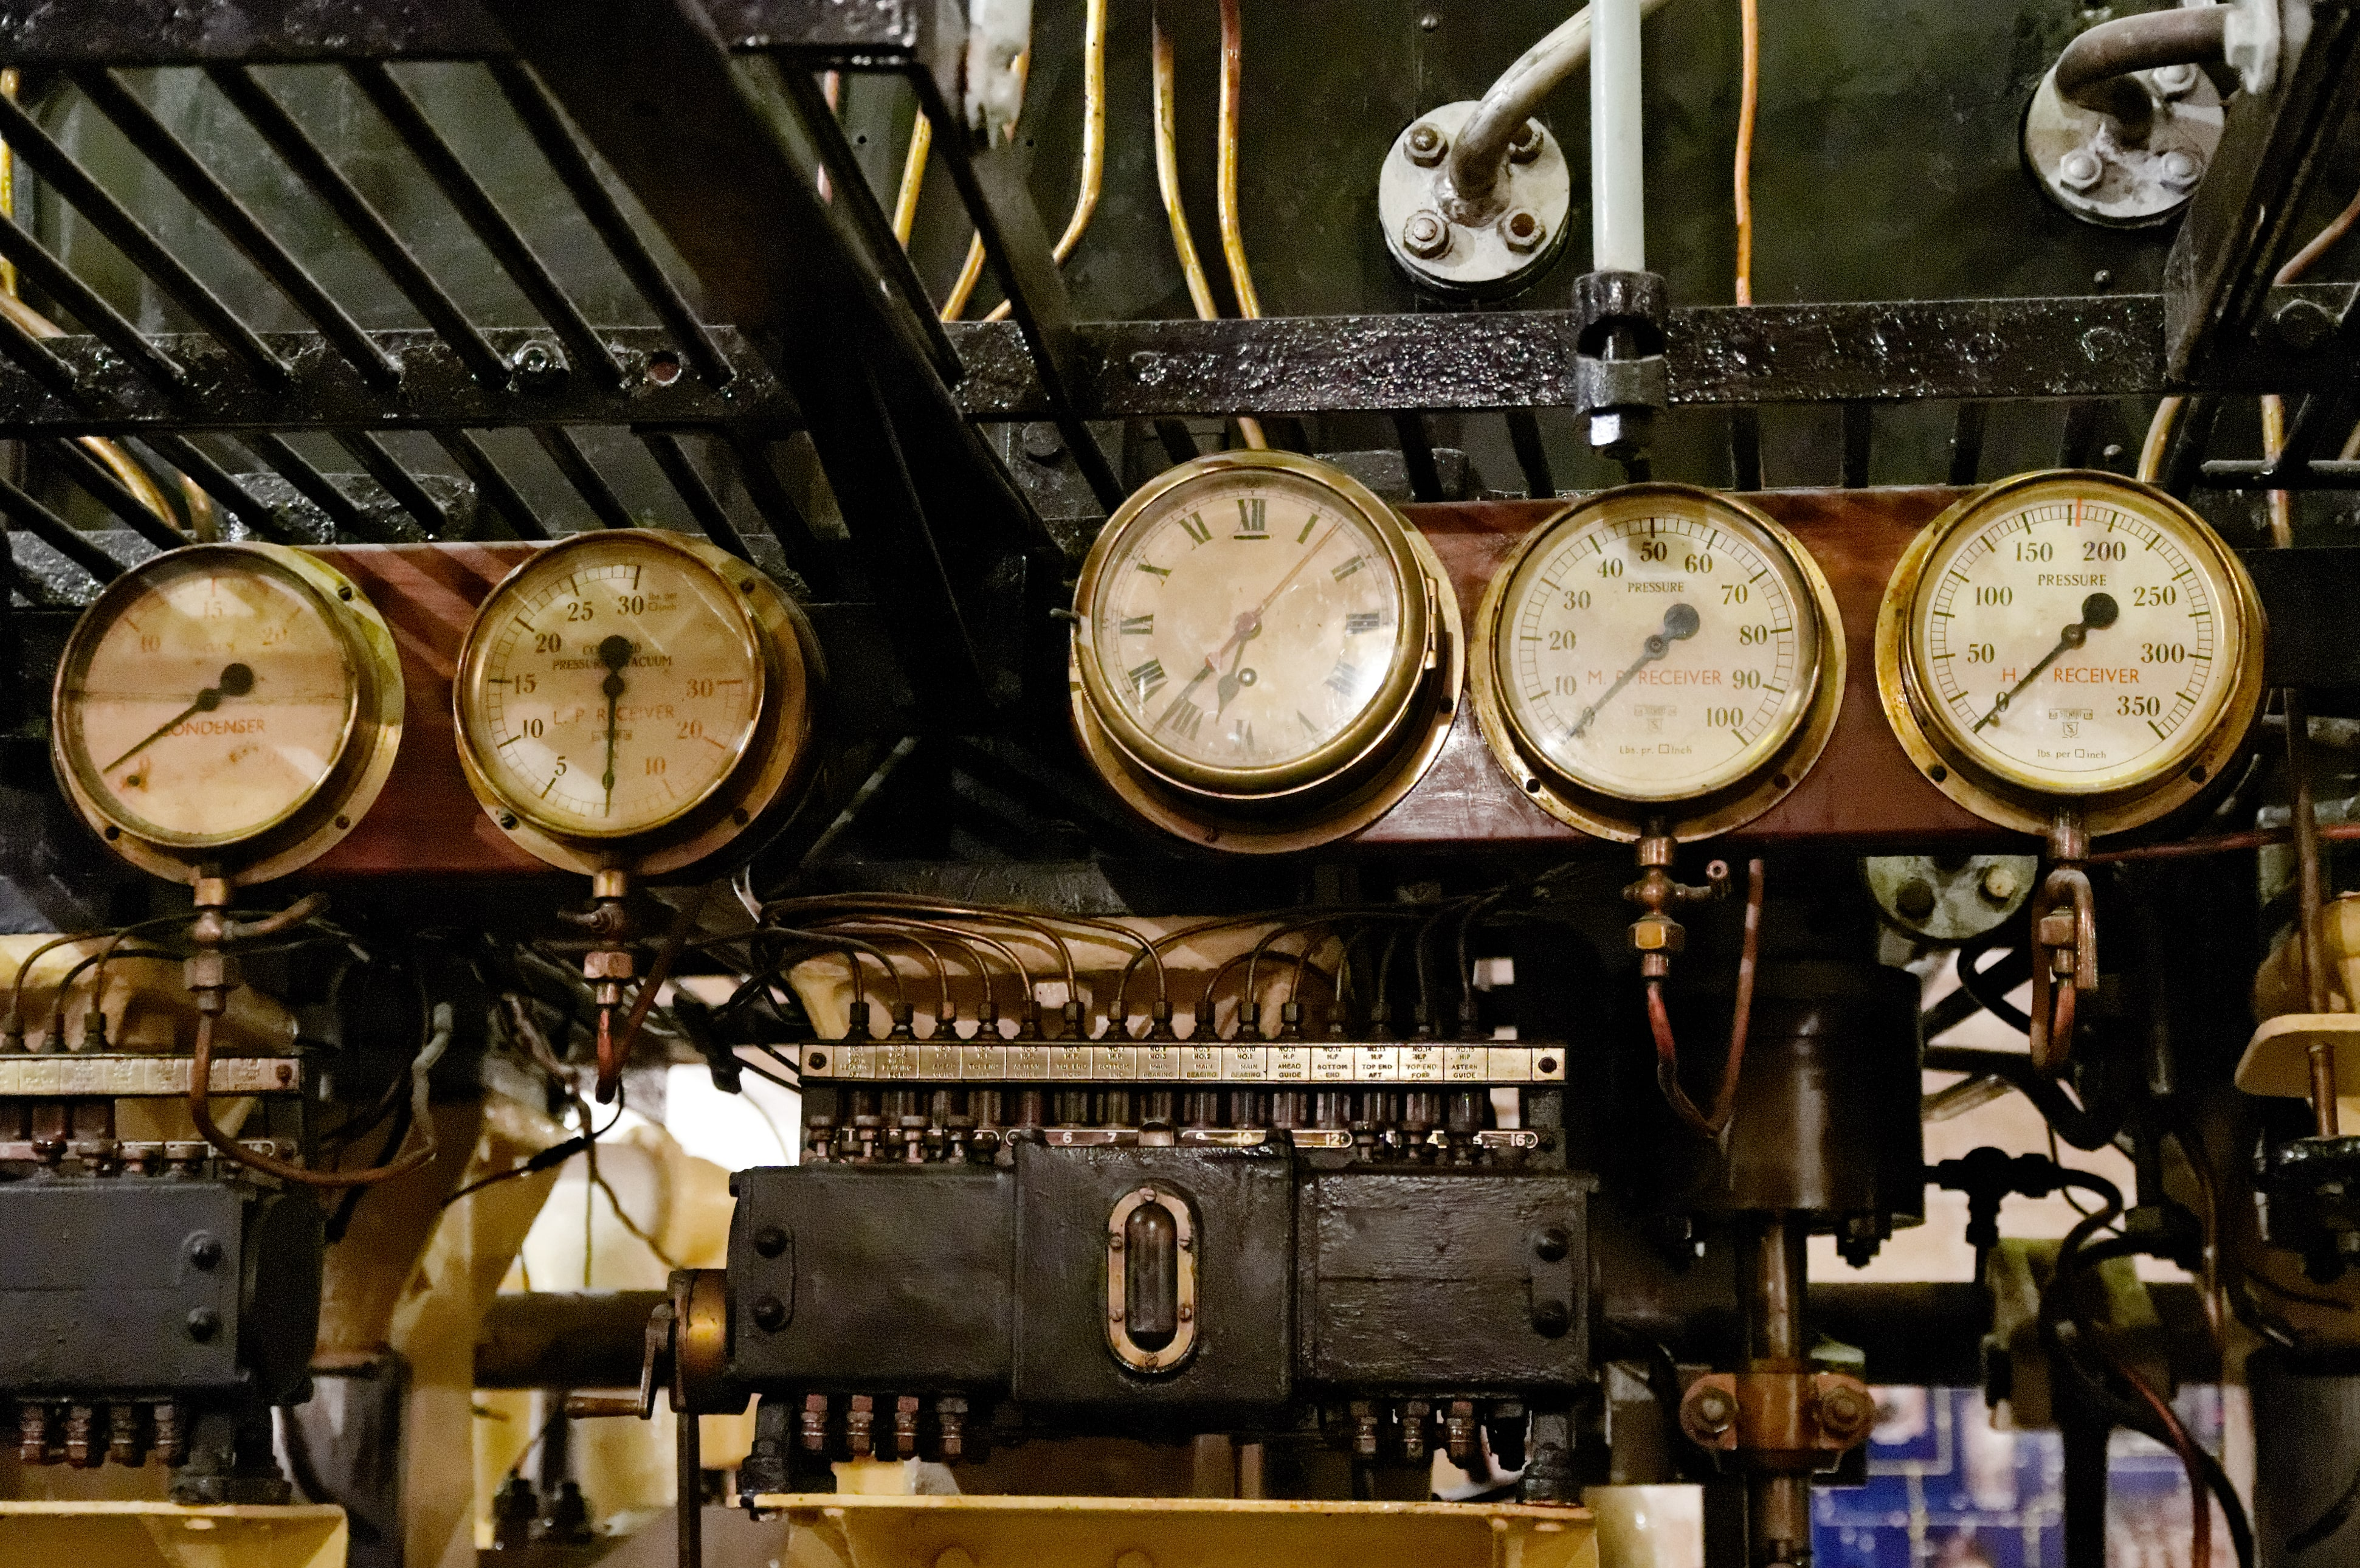
\includegraphics[width=\textwidth]{images/Intro/modernsteamengine.jpg}
        \caption{steam engine \cite{triple_expansion_engine}}
        \label{fig:modernsteamengine}
    \end{subfigure}
    \begin{subfigure}{0.3\textwidth}  % <----
        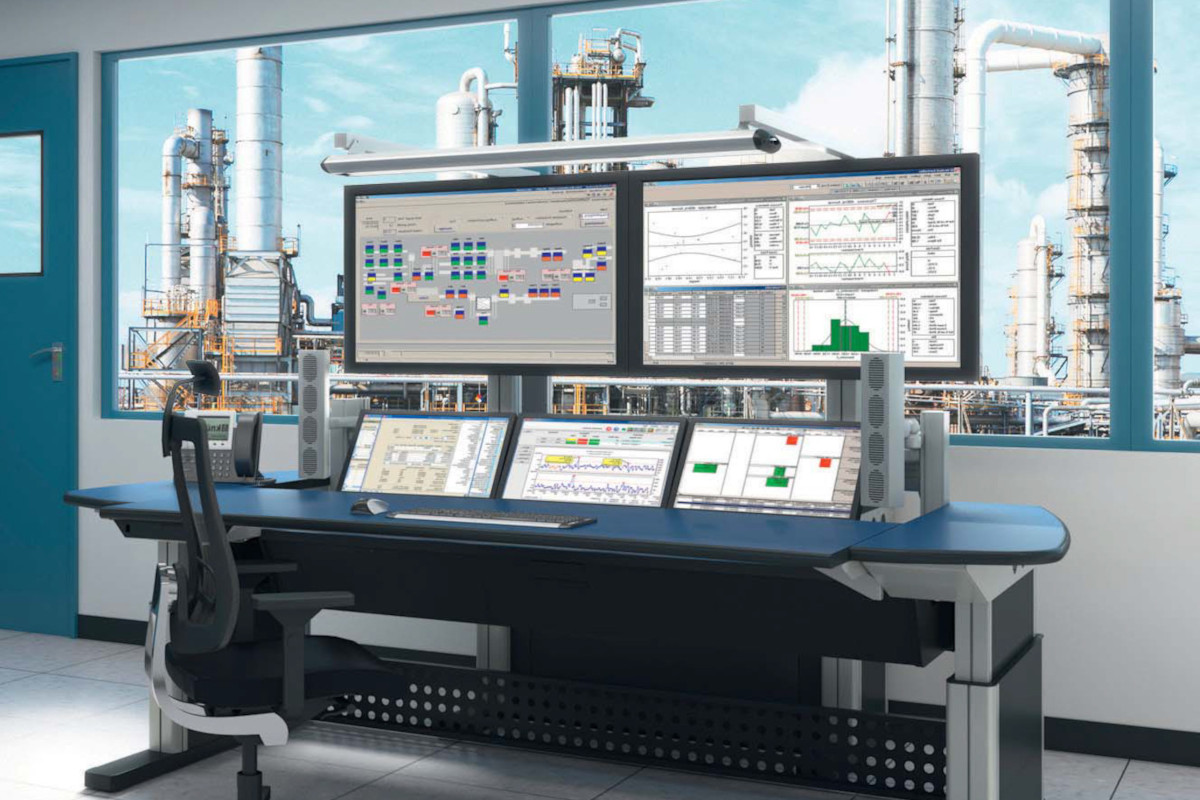
\includegraphics[width=\textwidth]{images/Intro/control-rooms-workstations.jpg}
        \caption{control room \cite{evosite}}
        \label{fig:controlroom}
    \end{subfigure}
    \caption{Evolution of machinery}
    \label{fig:machineryevolution}
\end{figure}

\paragraph*{}
The last comment is about where to run the algorithm. The most common approach is to run it on a server, that is not part of the device itself. This has the advantage of not having constraints on how much computational power is needed, because it's usually feasible to add more computational power to a computer that is not located on the device itself. The main drawback is that the data has to be transmitted to the server. This may not be feasible in some cases, for example for a mobile device, or for a device that is located in a remote area with no internet connection. In this case, the algorithm has to be run near the device itself, usually on a microcontroller that will perform an action when the algorithm detects a malfunction. This approach is called \emph{\gls{glo:edge}}. Using a microcontroller also has the advantage of requiring very little power, which is critical for battery-powered devices.


